\chapter*{Annexes}
\addcontentsline{toc}{chapter}{Annexes}

\section*{1. Schémas d'utilisation de l'ontologie}\label{annexe1}
\addcontentsline{toc}{section}{Schéma de base d'utilisation de l'ontologie}
\begin{figure} [H]
    \centering
    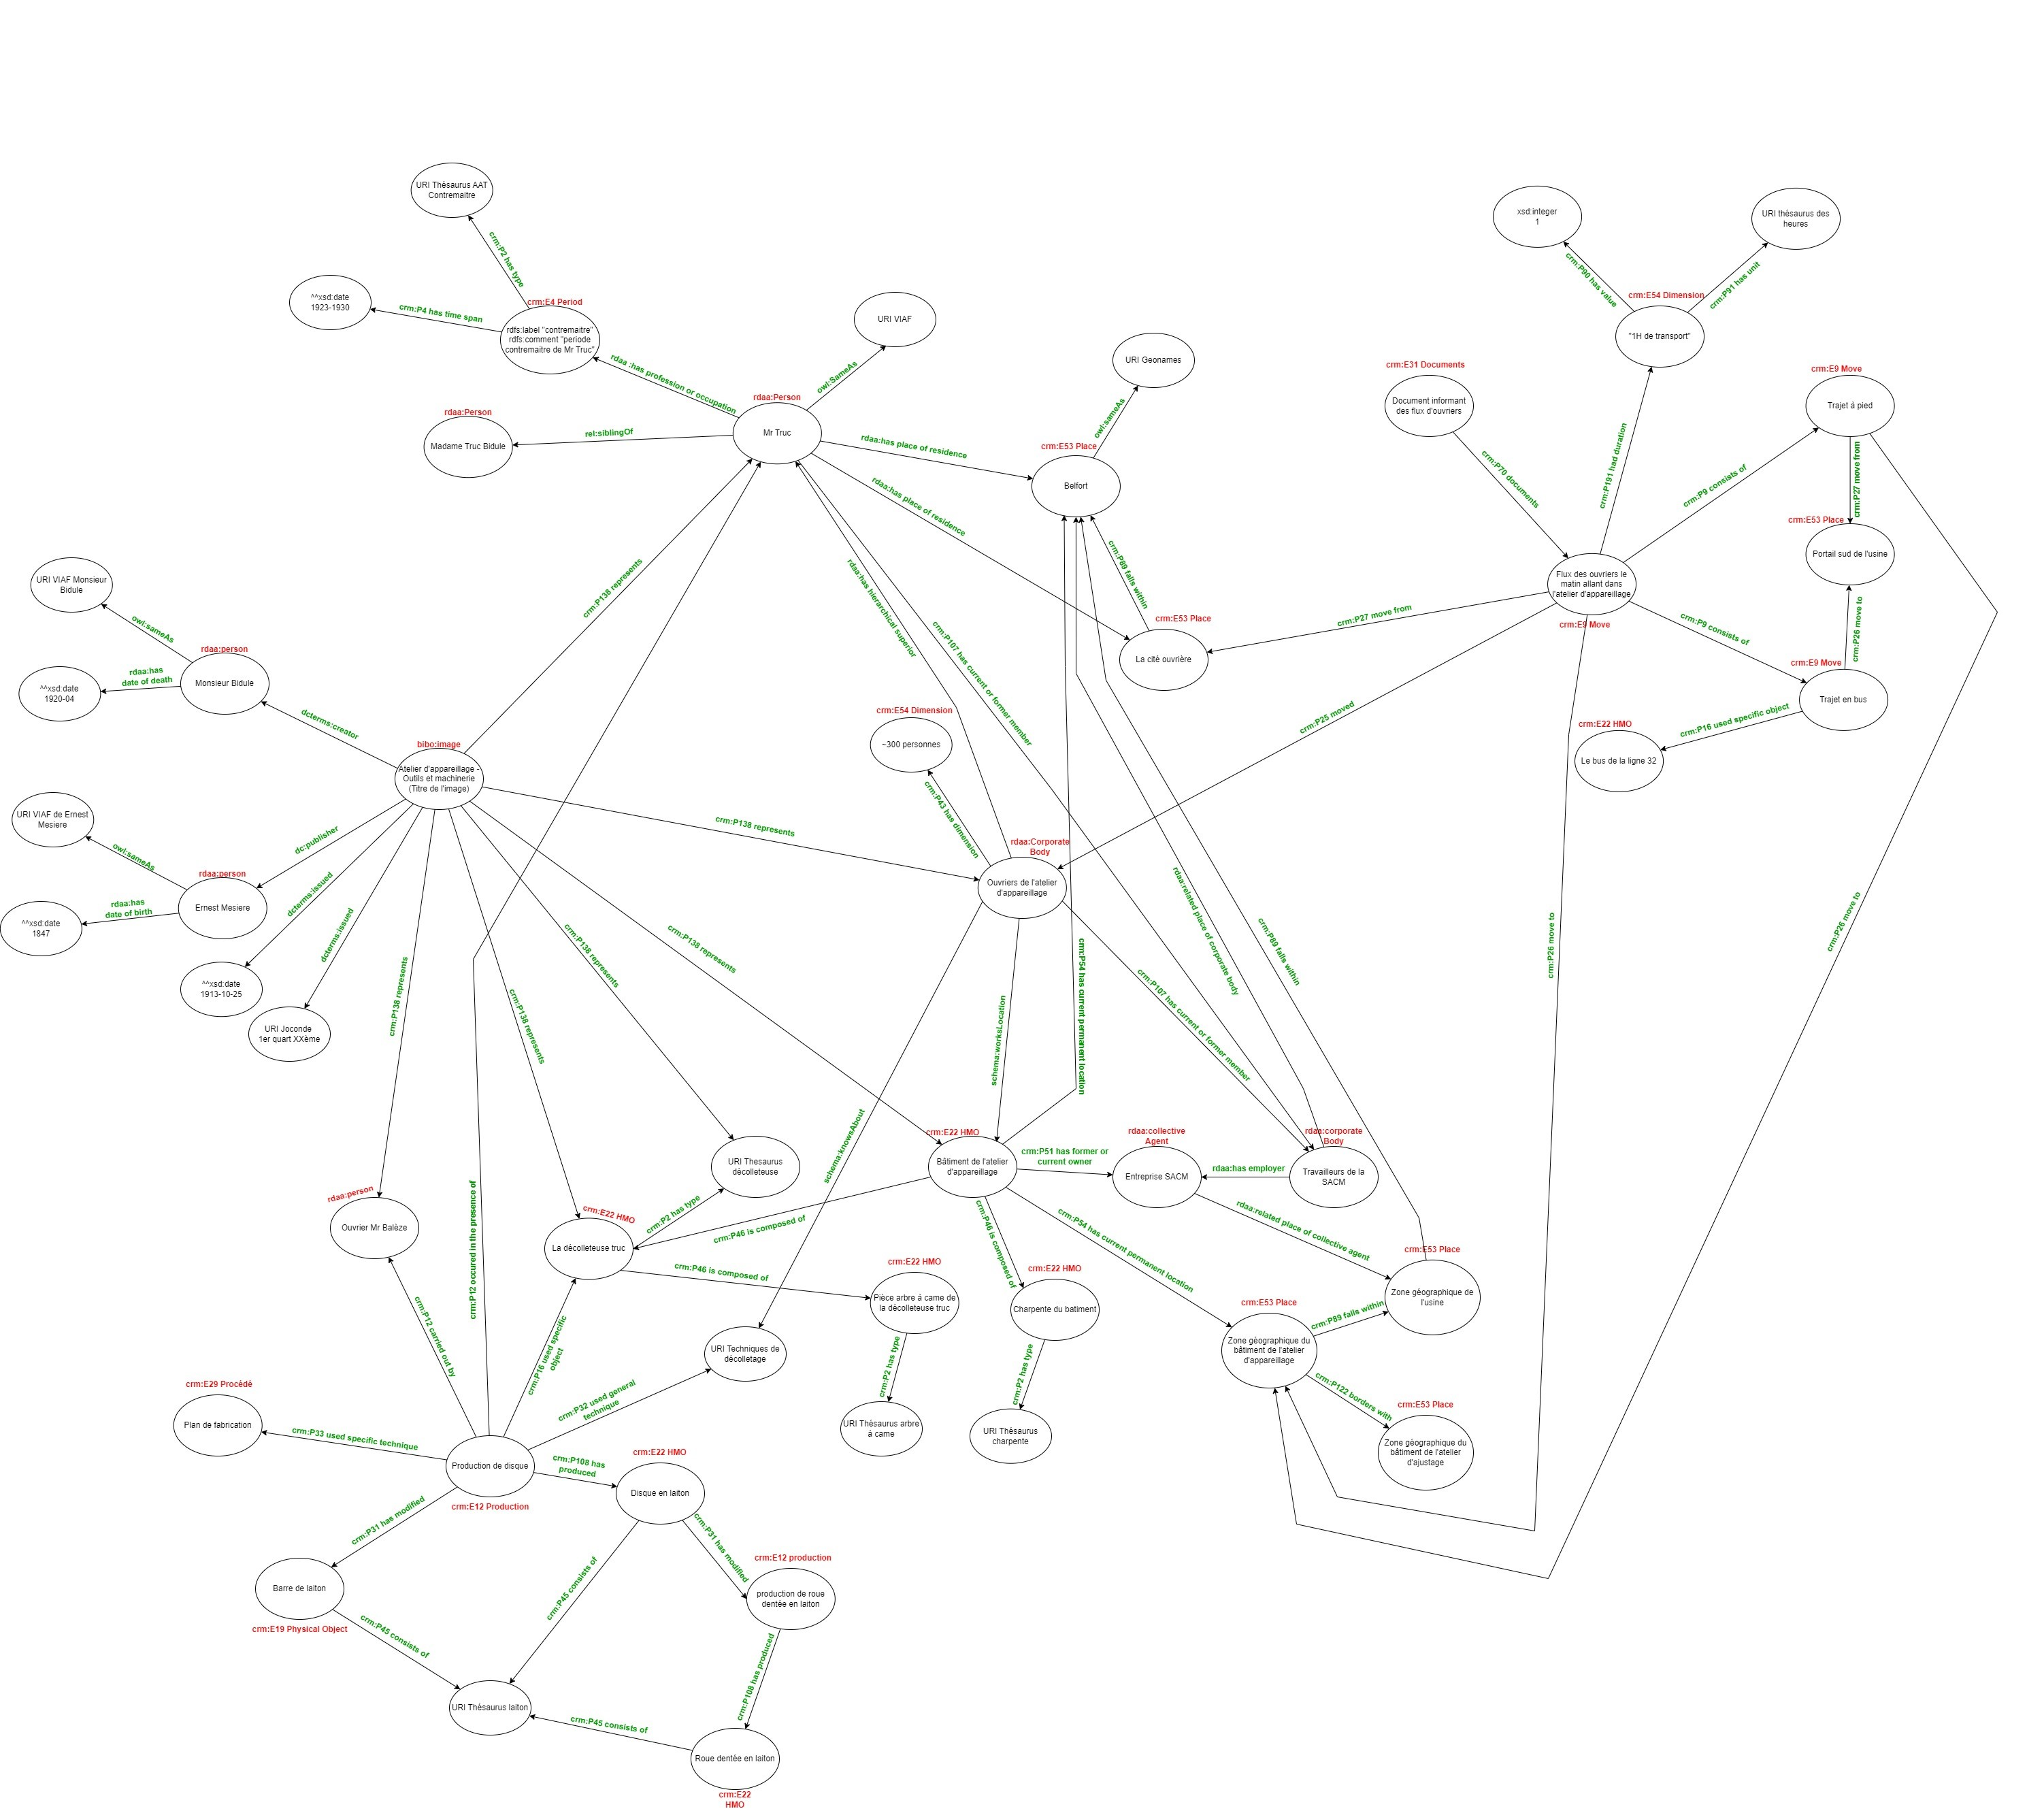
\includegraphics[width=1\textwidth]{assets/annexes/schema_base_ontologie_TTM.jpg}
    \caption{Schéma de base décrivant l'utilisation de l'ontologie dédiée au projet}
    \label{fig:schemaBaseTTM}
\end{figure}

\addcontentsline{toc}{section}{Schéma décrivant la production de fil de coton à l'aide du Manuel Roret}
\begin{figure} [H]
    \centering
    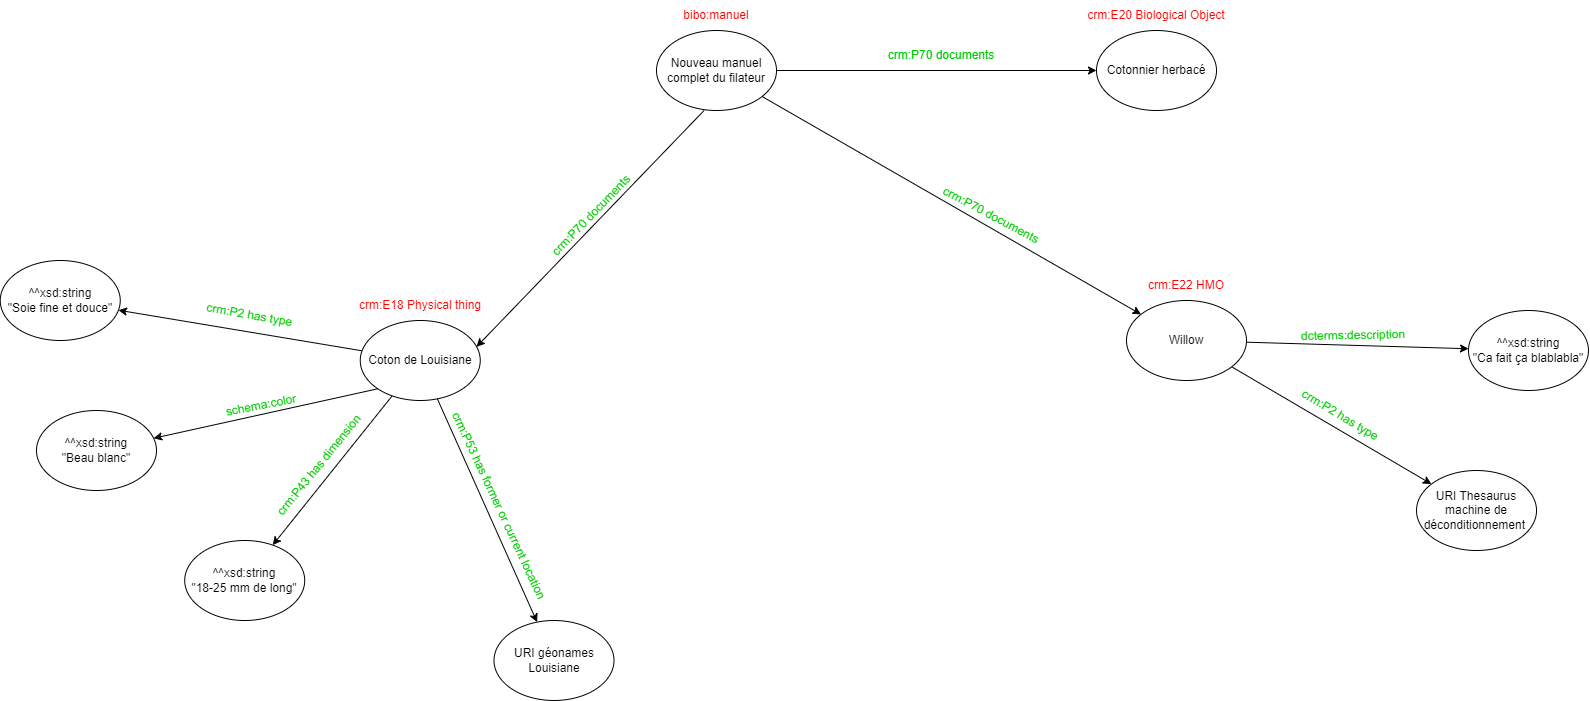
\includegraphics[width=1\textwidth]{assets/annexes/schema_manuel_roret.png}
    \caption{Schéma décrivant la production de fil de coton à l'aide du Manuel Roret}
    \label{fig:schemaRoretTTM}
\end{figure}

\addcontentsline{toc}{section}{Schéma décrivant les murs des bâtiments du Techn'hom}
\begin{figure} [H]
    \centering
    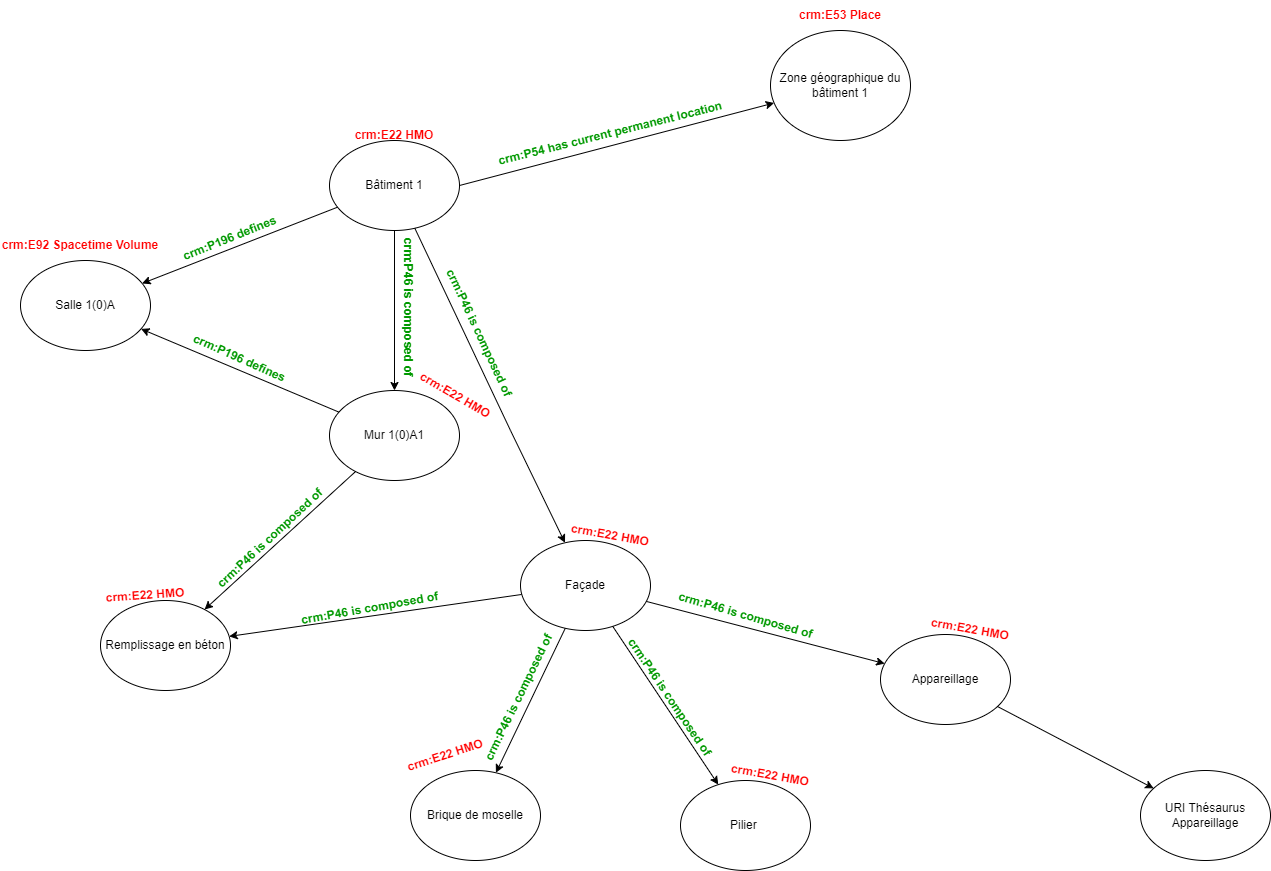
\includegraphics[width=1\textwidth]{assets/annexes/schema_desciption_mur.png}
    \caption{Schéma décrivant les murs des bâtiments du Techn'hom}
    \label{fig:schemaMursTTM}
\end{figure}

\section*{2. Graphe modélisant les relations entre ontologie}\label{annexe2}
\addcontentsline{toc}{section}{Graphe modélisant les relations entre ontologie}
\begin{figure} [H]
    \centering
    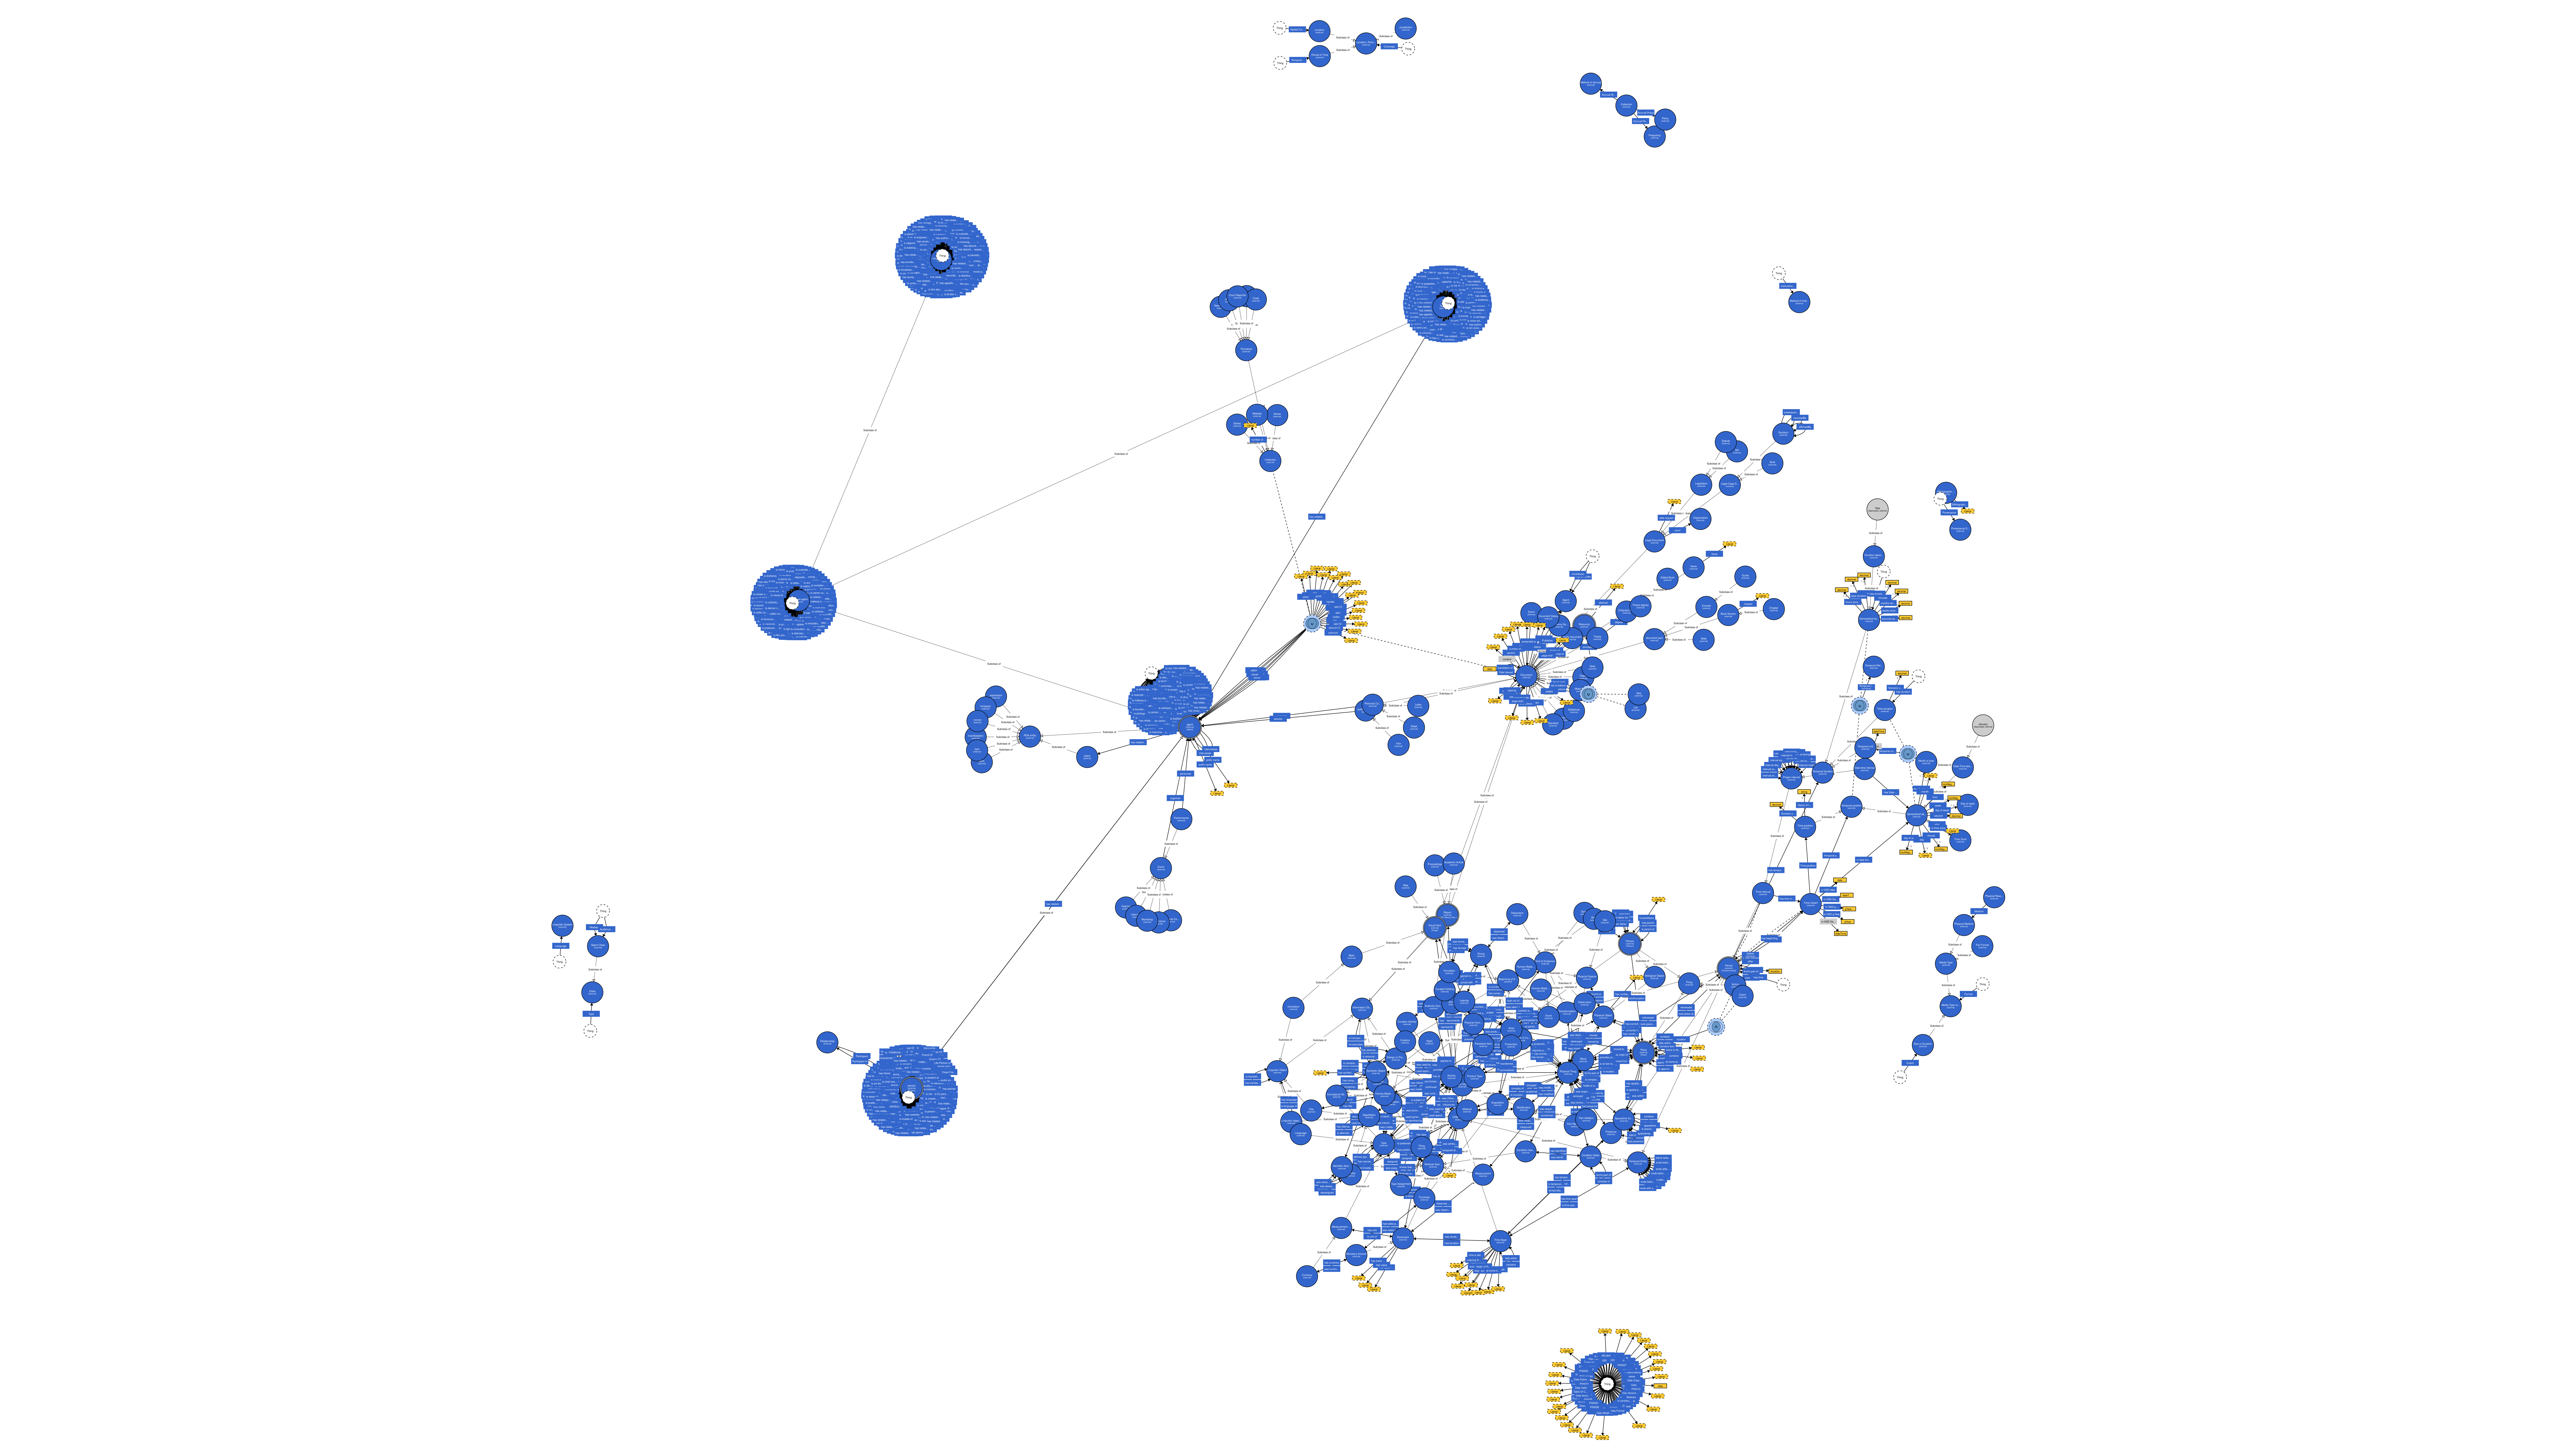
\includegraphics[width=1\textwidth]{assets/annexes/scheam_decla_ontologie.png}
    \caption{Graphe modélisant les relations théoriques entre ontologie}
    \label{fig:schemaGrapheOntologie}
\end{figure}

\section*{3. Application Omeka-S (vue site web)}\label{annexe3}
\addcontentsline{toc}{section}{Application Omeka-s (vue site web) - Page "Projet"}
\begin{figure} [H]
    \centering
    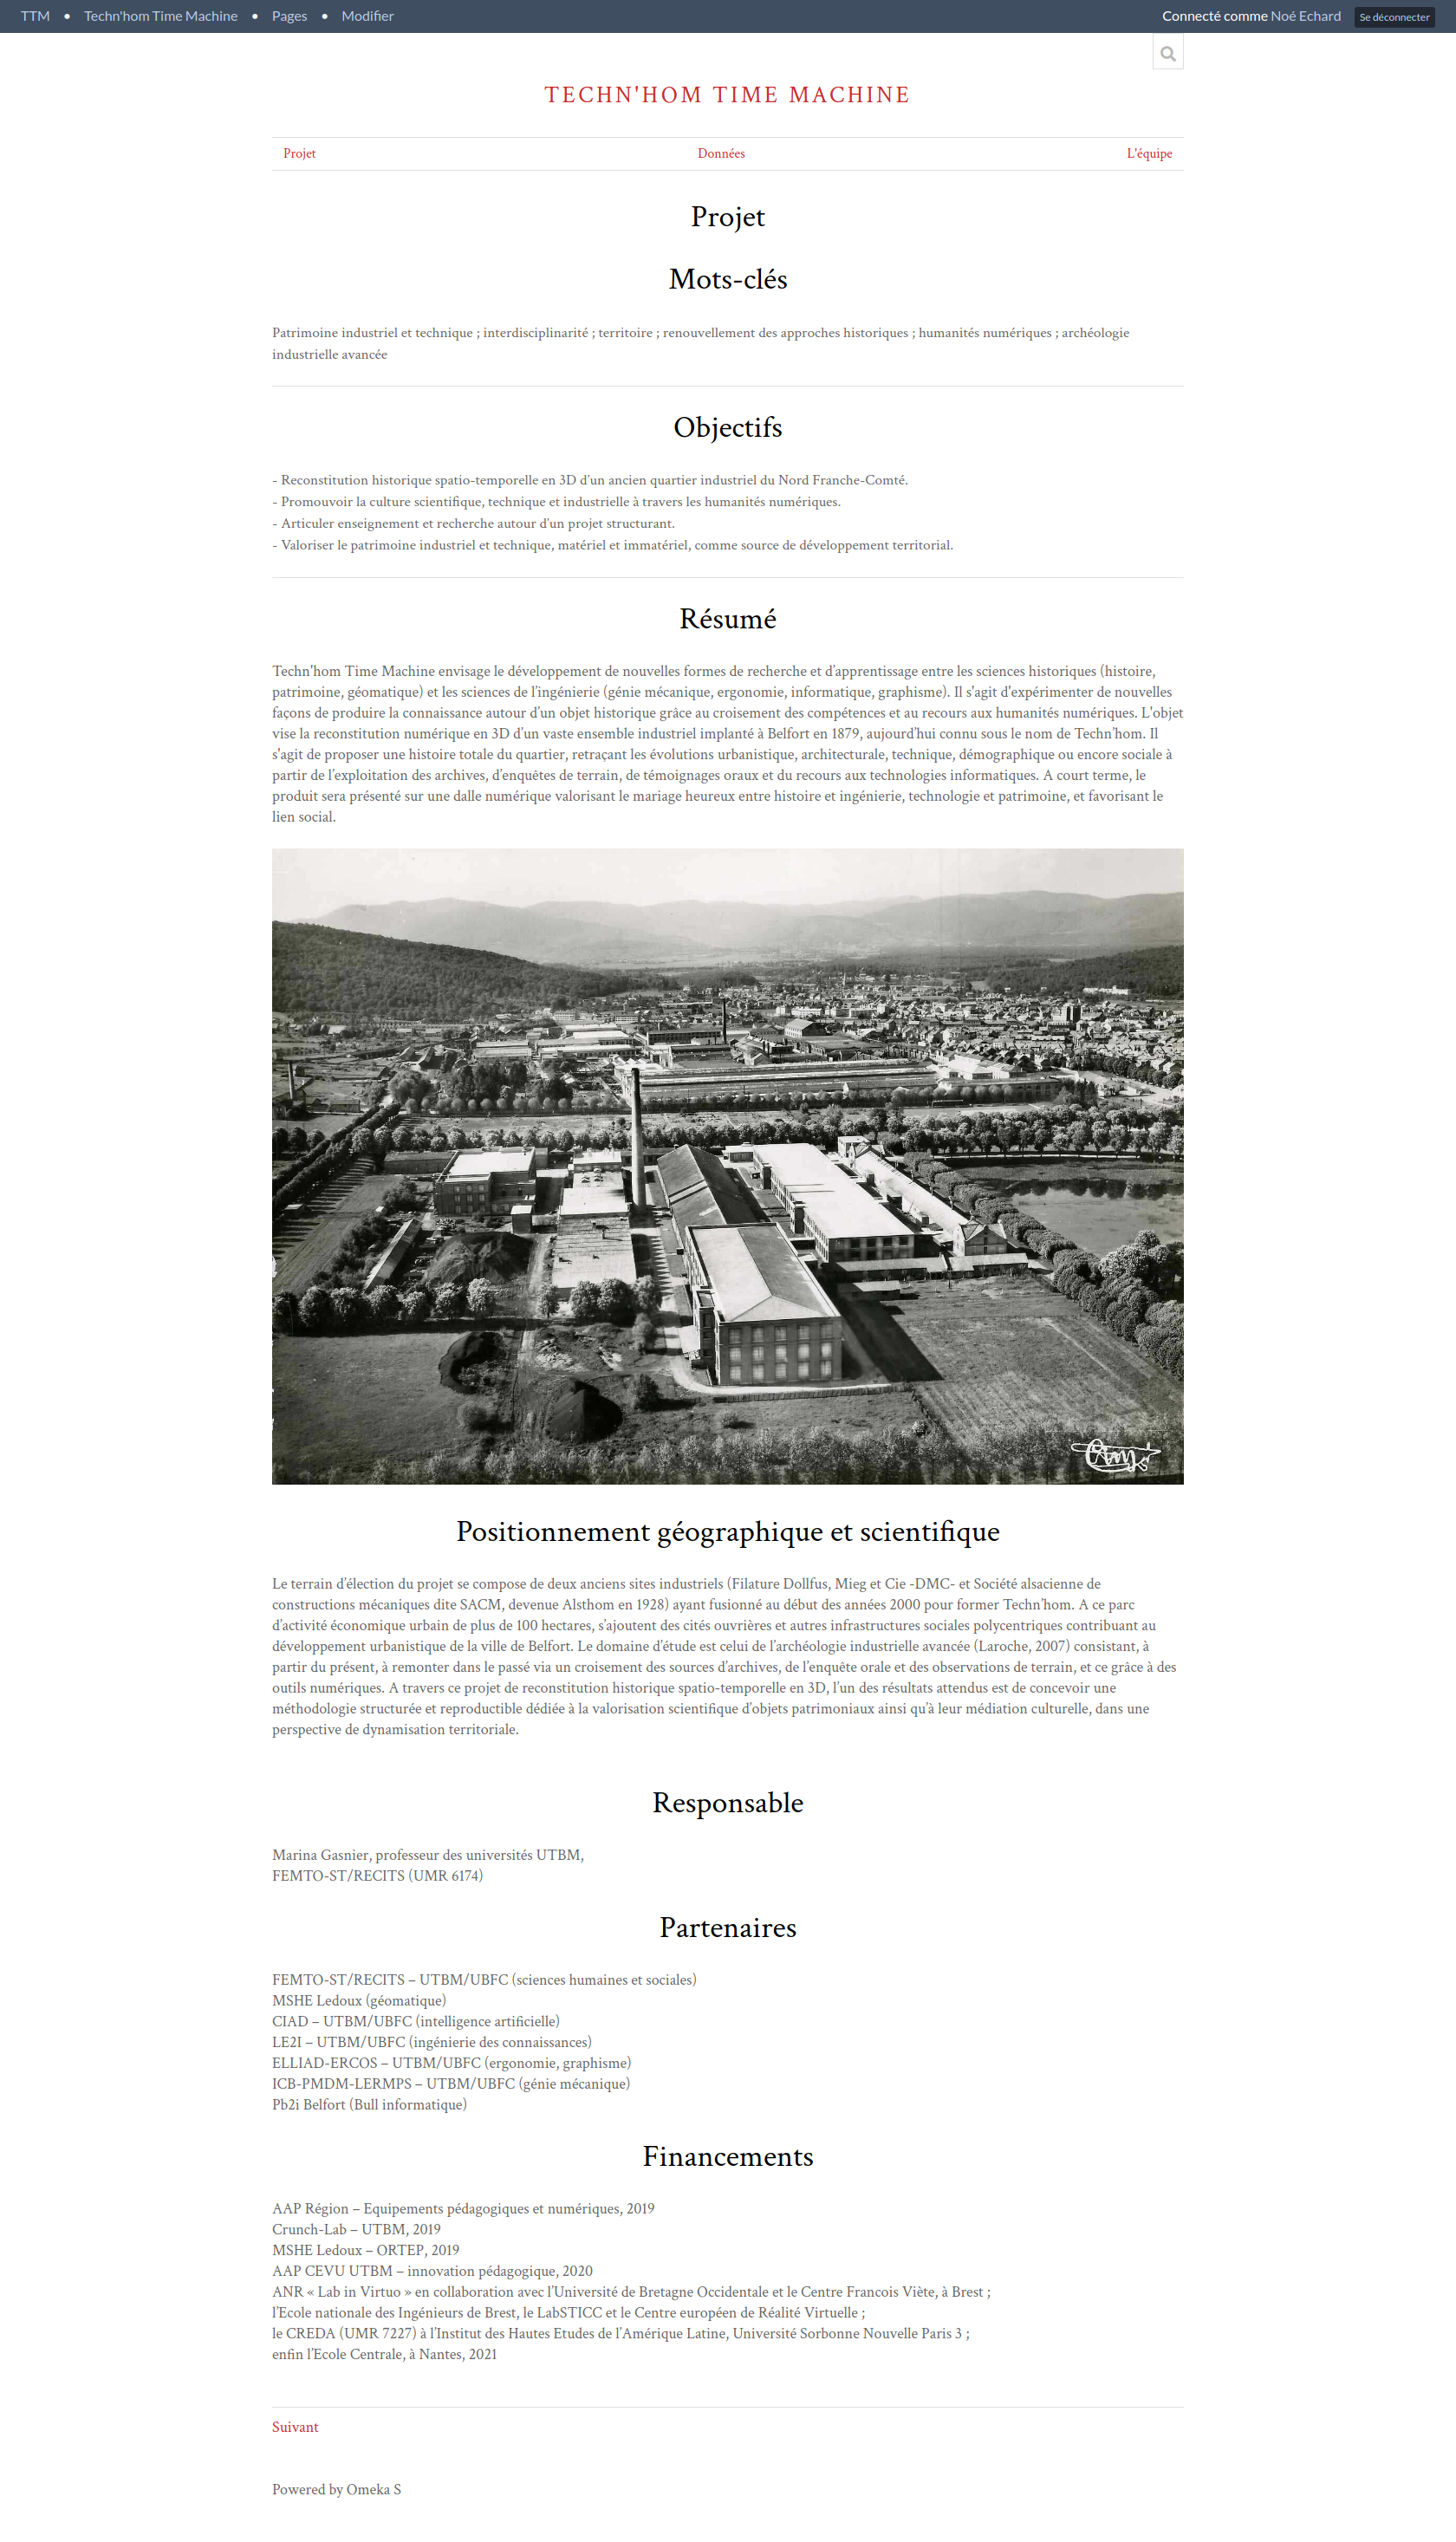
\includegraphics[width=0.8\textwidth]{assets/annexes/omeka_projet.png}
    \caption{Capture d'écran de la page "Projet" du site web du projet}
    \label{fig:pageProjetOmeka}
\end{figure}
\addcontentsline{toc}{section}{Application Omeka-s (vue site web) - Page "Equipe"}
\begin{figure} [H]
    \centering
    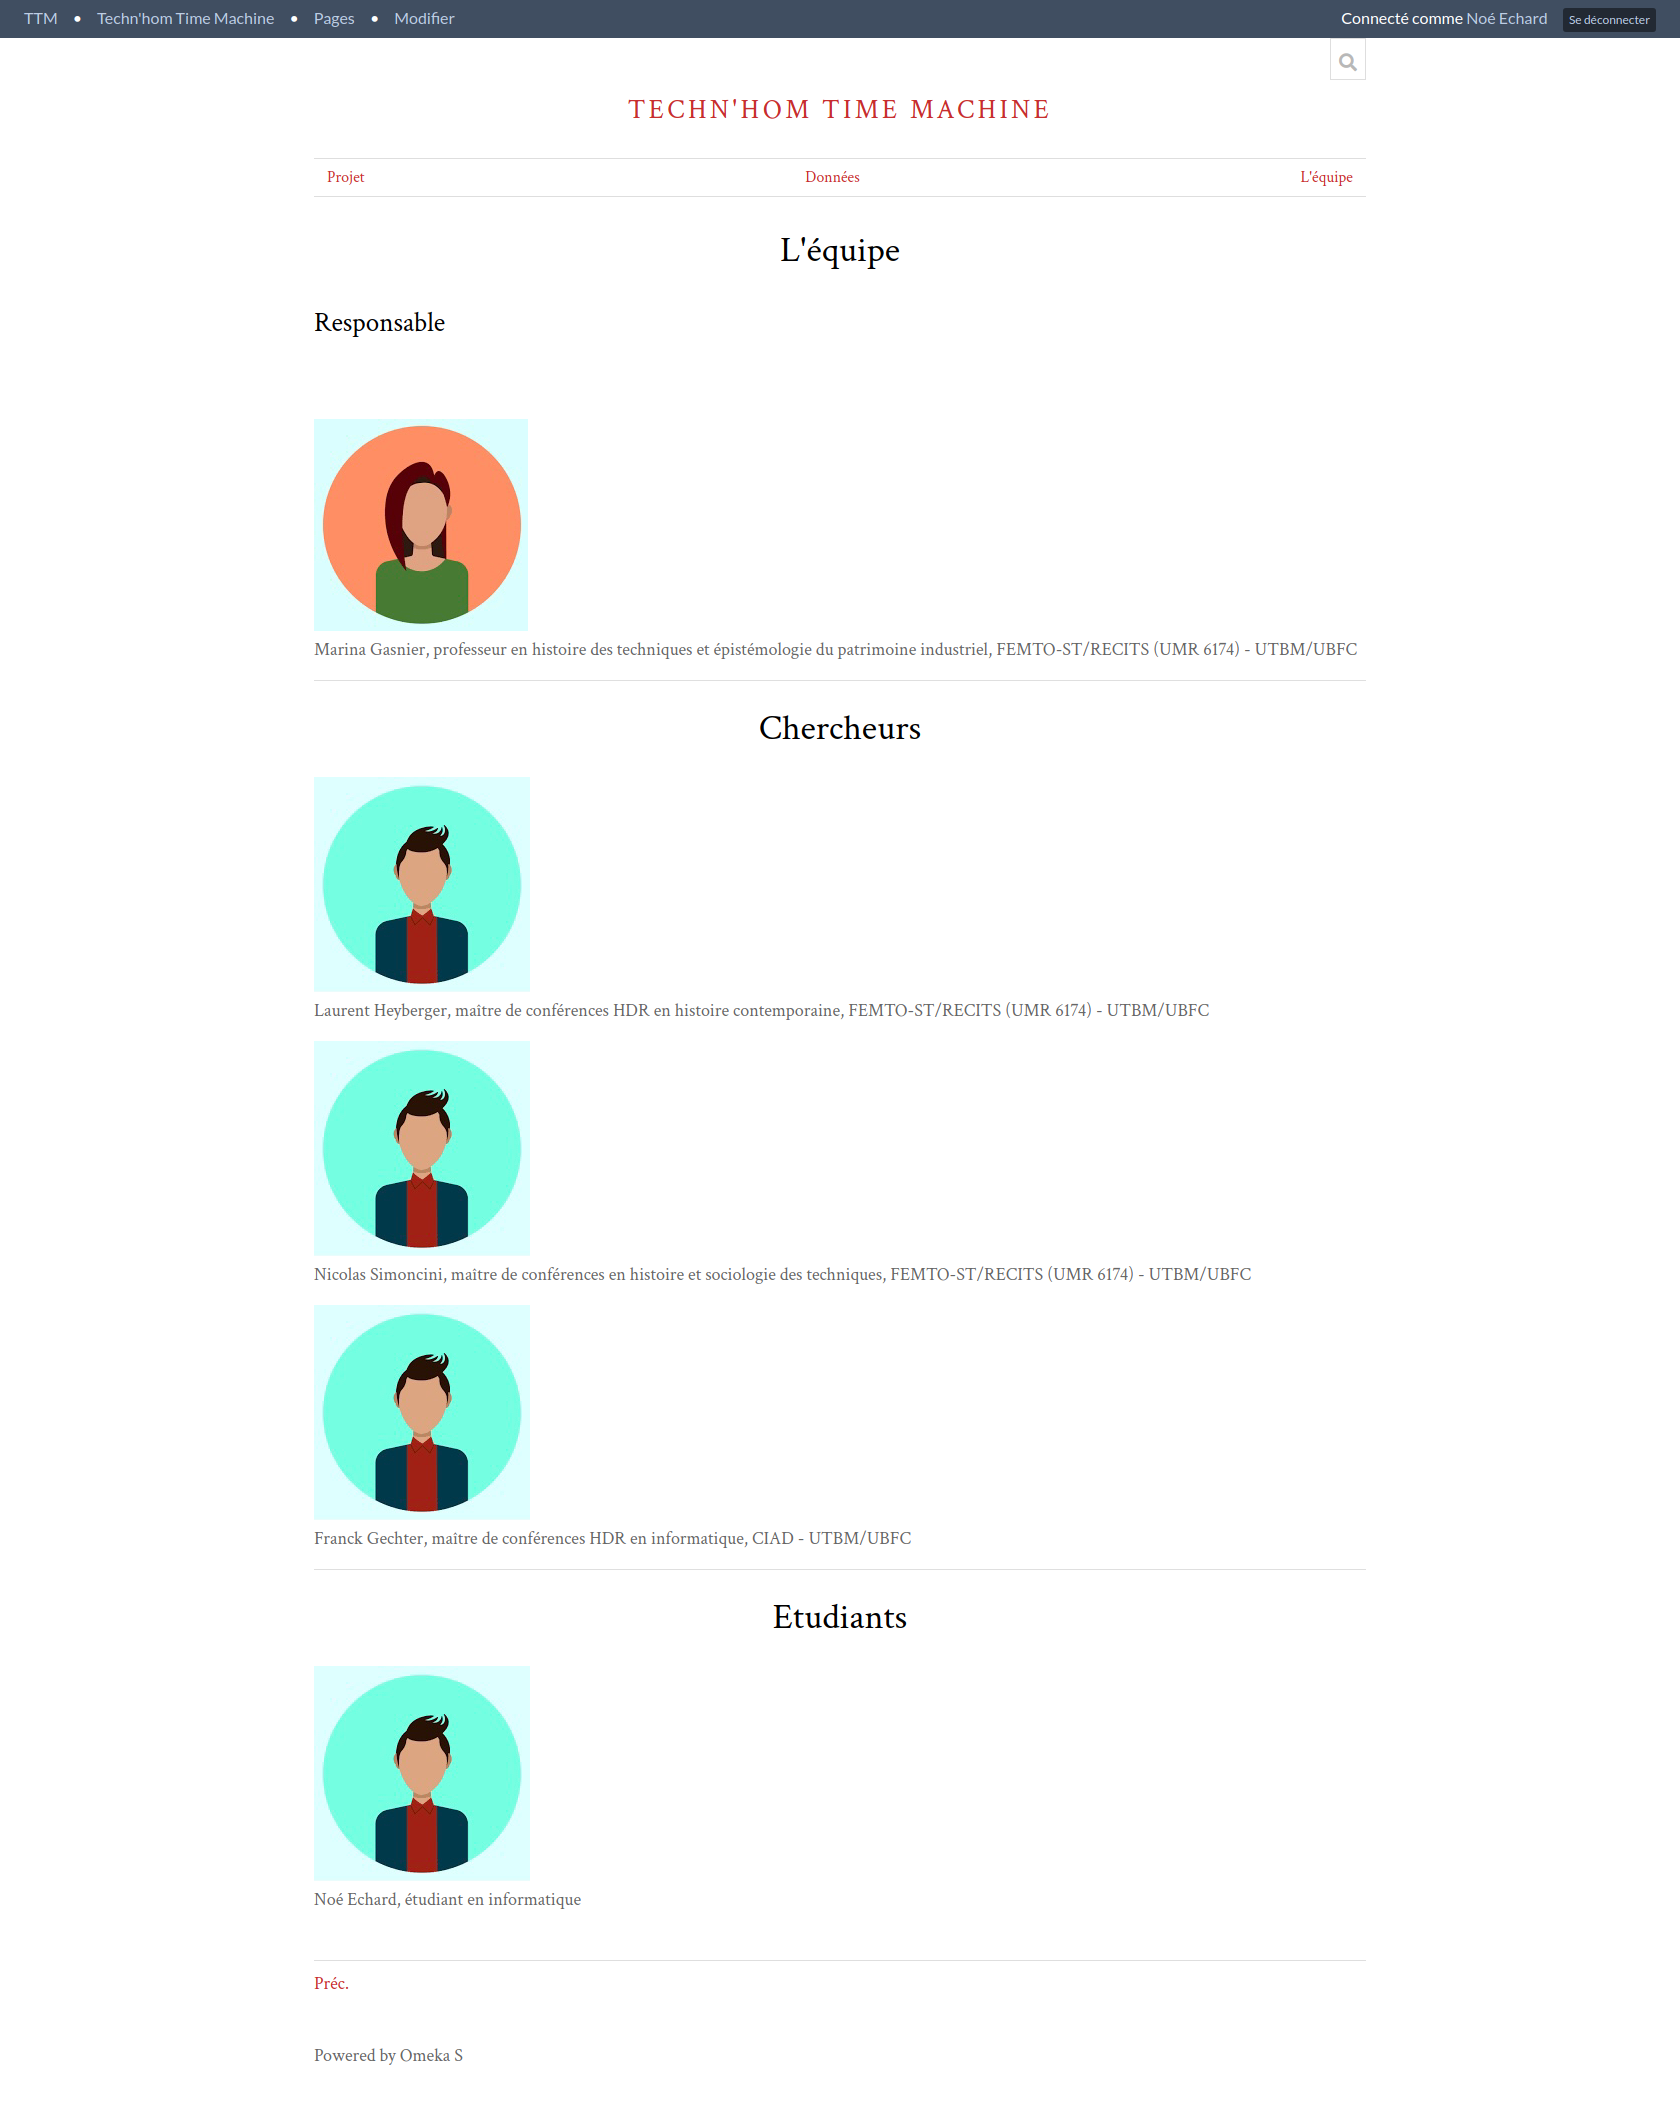
\includegraphics[width=1\textwidth]{assets/annexes/omeka_equipe.png}
    \caption{Capture d'écran de la page "Equipe" du site web du projet}
    \label{fig:pageEquipeOmeka}
\end{figure}
\addcontentsline{toc}{section}{Application Omeka-s (vue site web) - Page "Données"}
\begin{figure} [H]
    \centering
    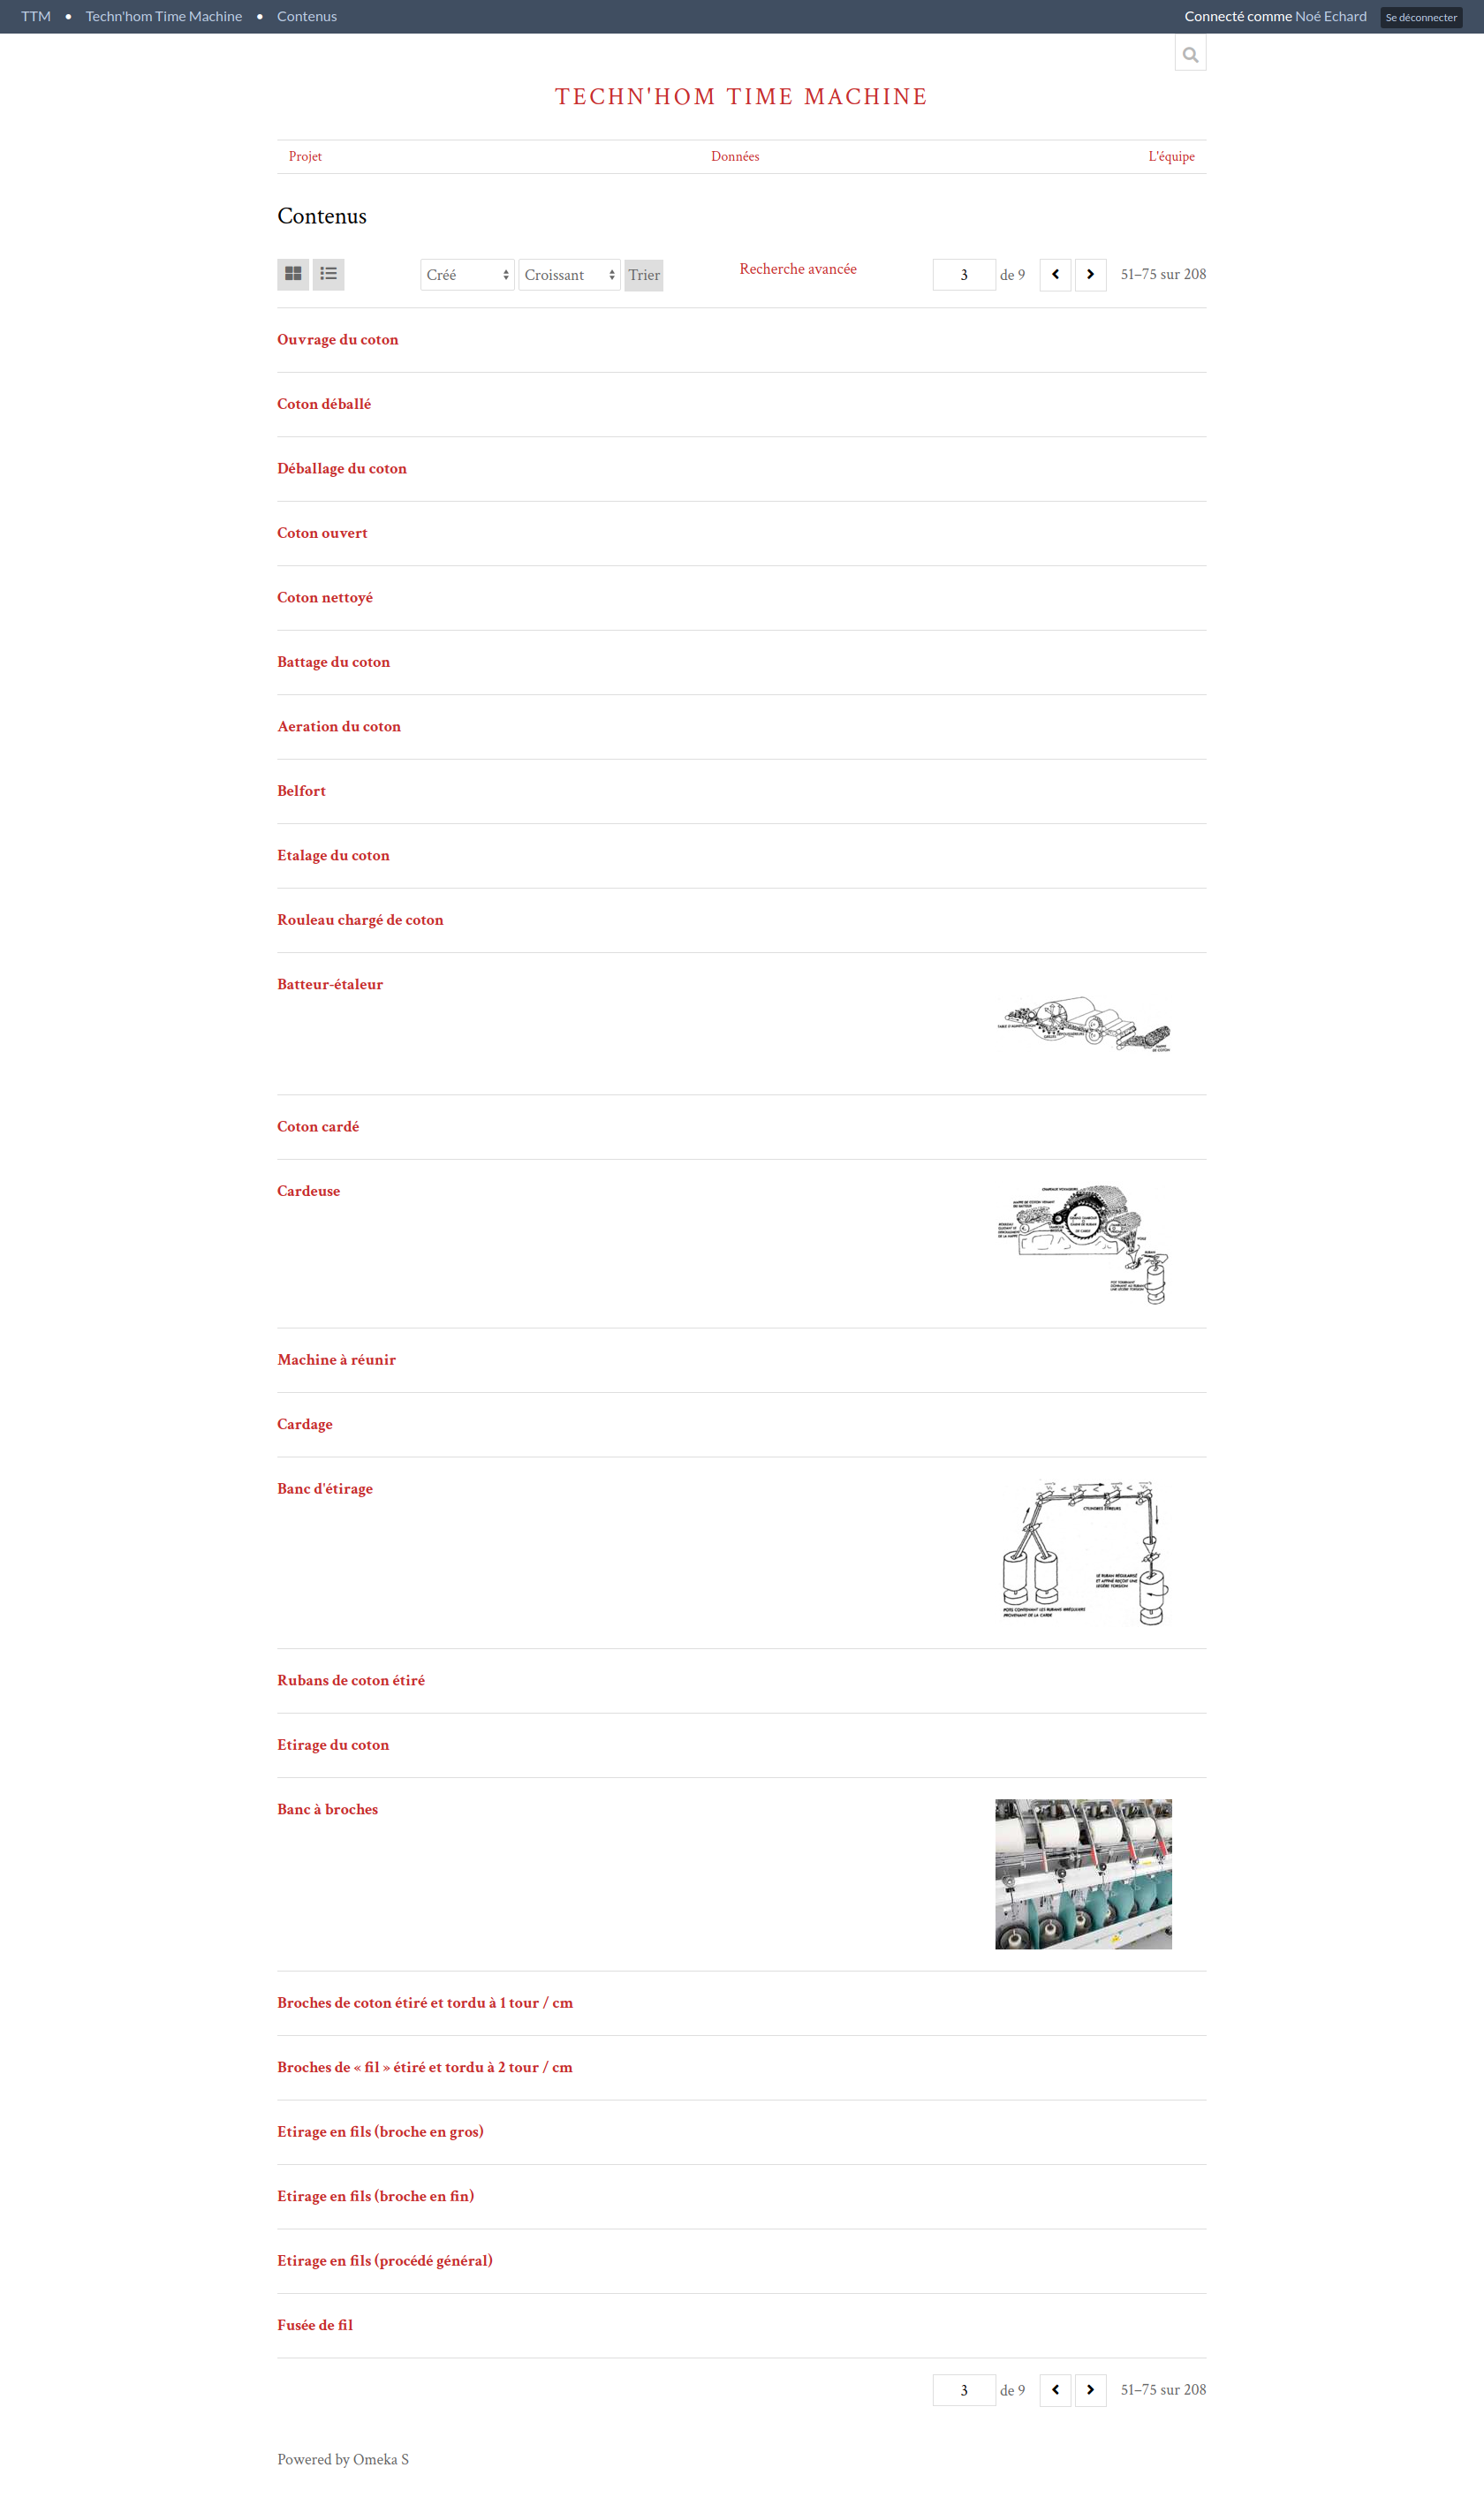
\includegraphics[width=0.8\textwidth]{assets/annexes/omeka_items.png}
    \caption{Capture d'écran de la page "Données" du site web du projet}
    \label{fig:pageDonnéesOmeka}
\end{figure}
\addcontentsline{toc}{section}{Application Omeka-s (vue site web) - Page de détail d'un item}
\begin{figure} [H]
    \centering
    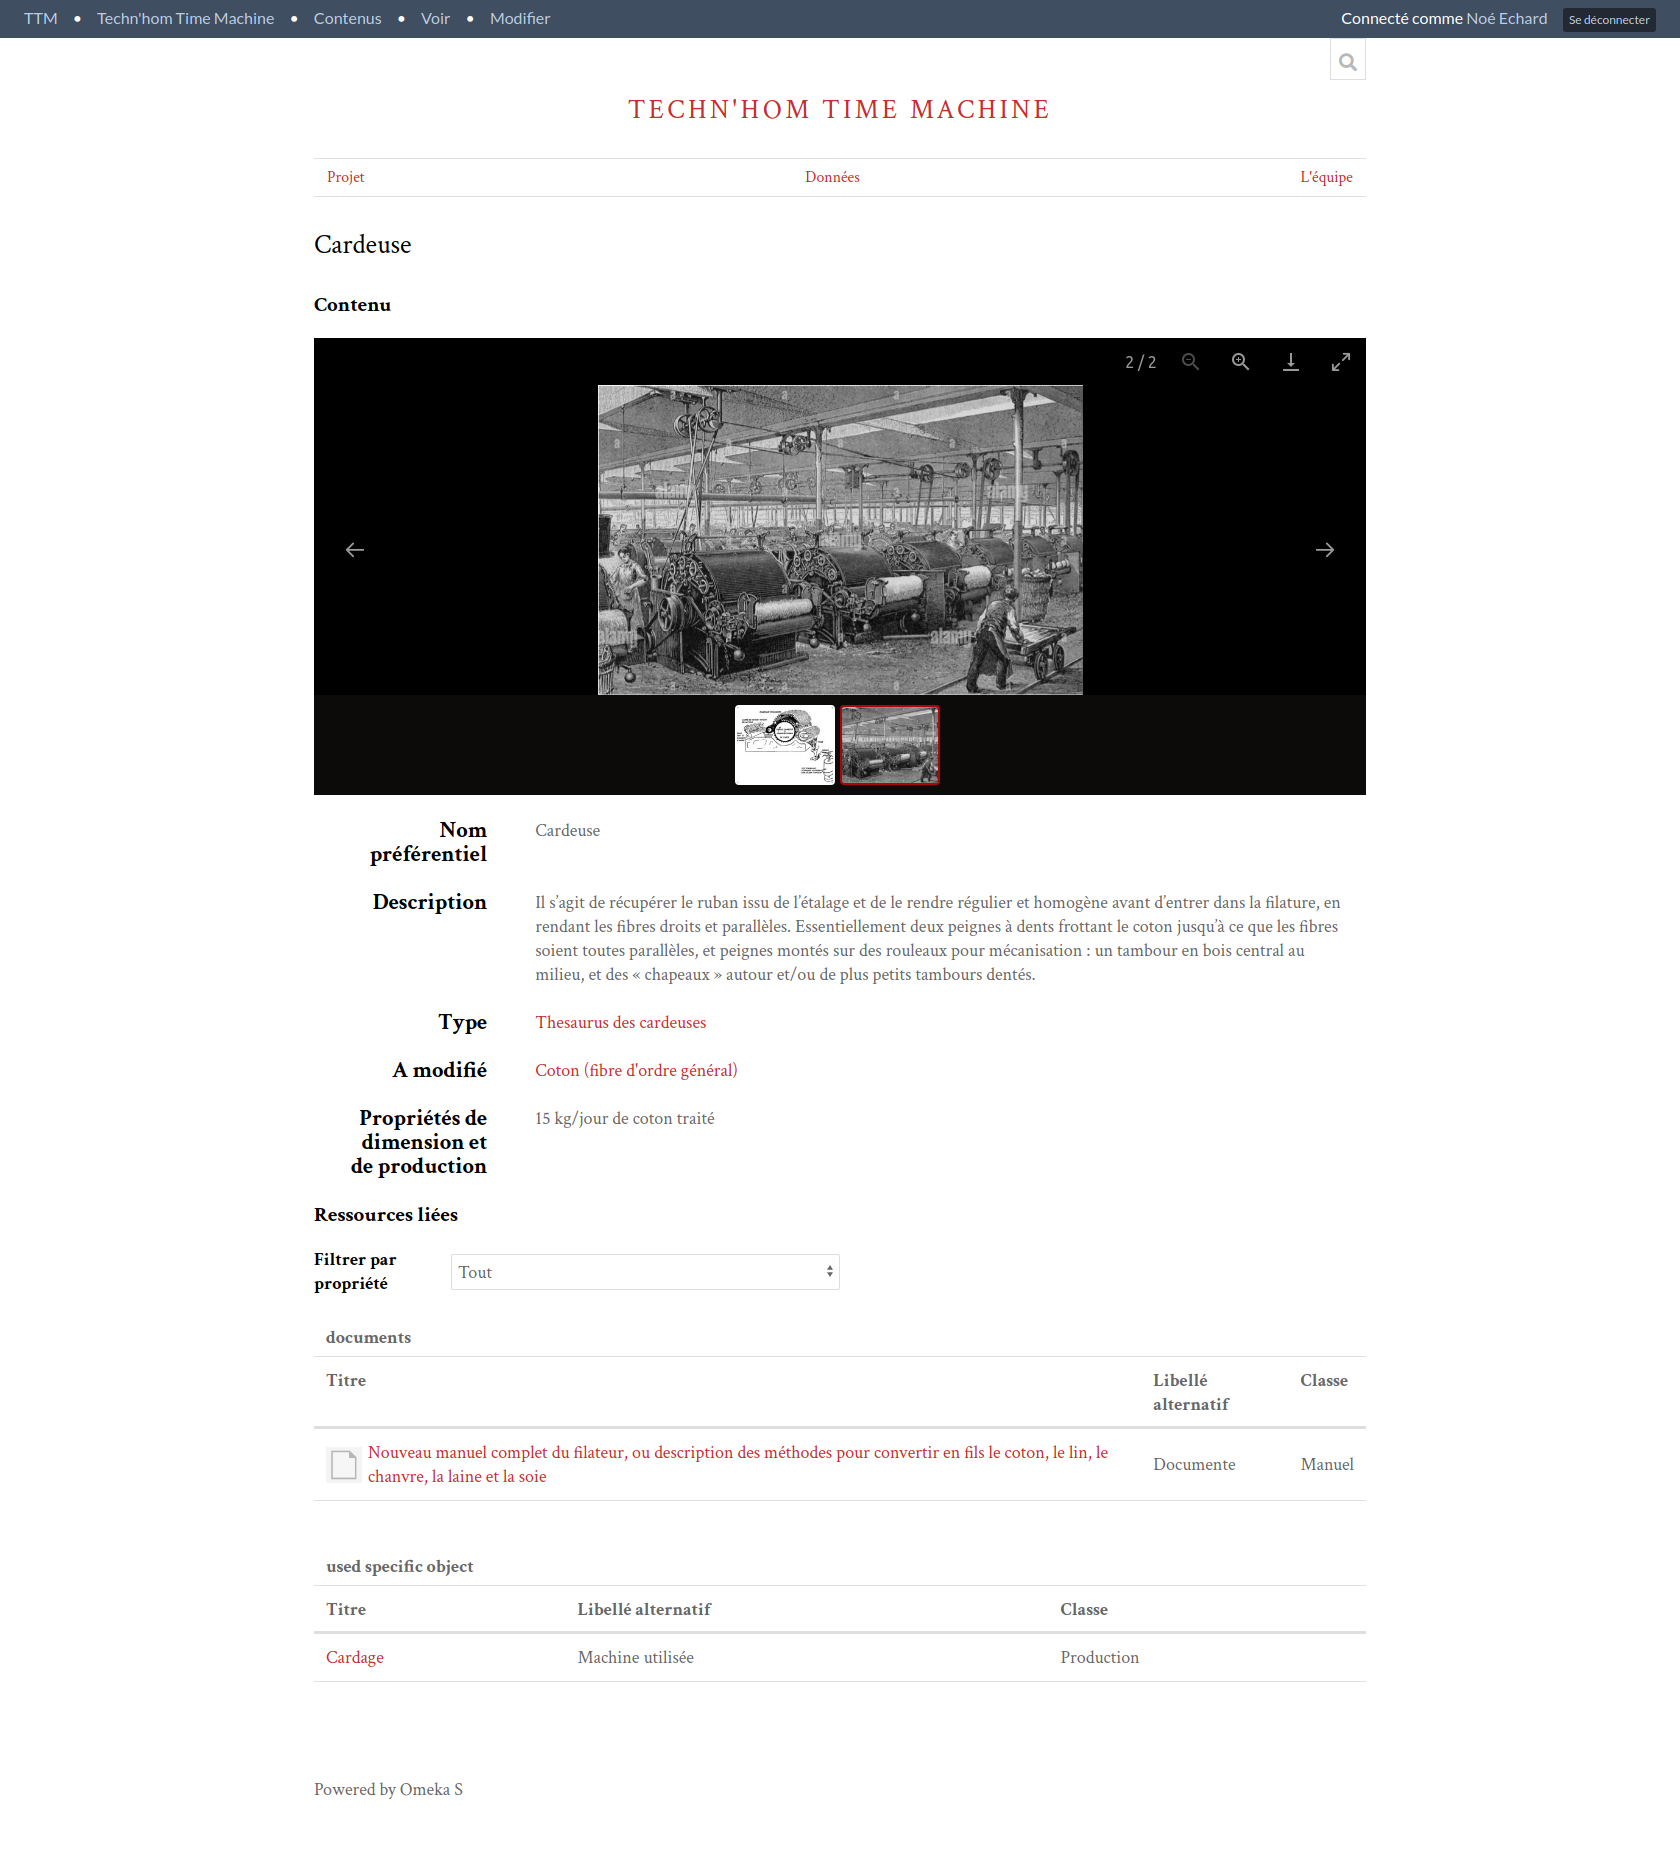
\includegraphics[width=0.8\textwidth]{assets/annexes/omeka_details.png}
    \caption{Capture d'écran de la page de détail d'un item du site web du projet}
    \label{fig:detailItemOmeka}
\end{figure}

\section*{4. Omeka-S}\label{annexe4}
\addcontentsline{toc}{section}{Omeka-S - Onglet "Contenus"}
\begin{figure} [H]
    \centering
    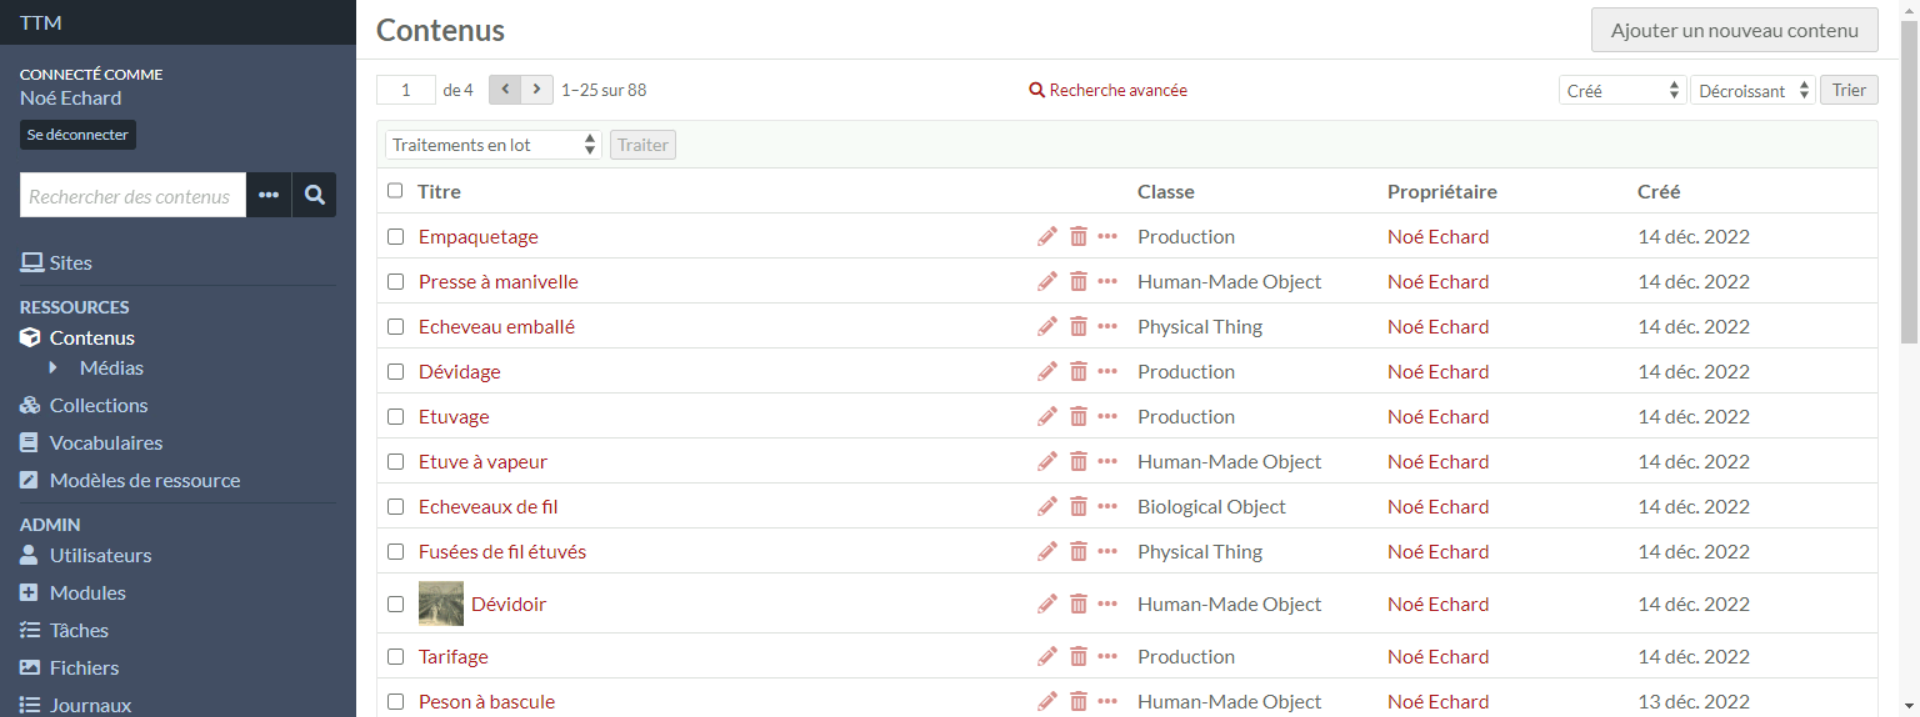
\includegraphics[width=1\textwidth]{assets/omeka/onglet_contenu_omeka.png}
    \caption{Capture d'écran de l'onglet contenus de Omeka-S}
    \label{fig:pageContenusOmeka}
\end{figure}

\addcontentsline{toc}{section}{Omeka-S - Onglet "Medias"}
\begin{figure} [H]
    \centering
    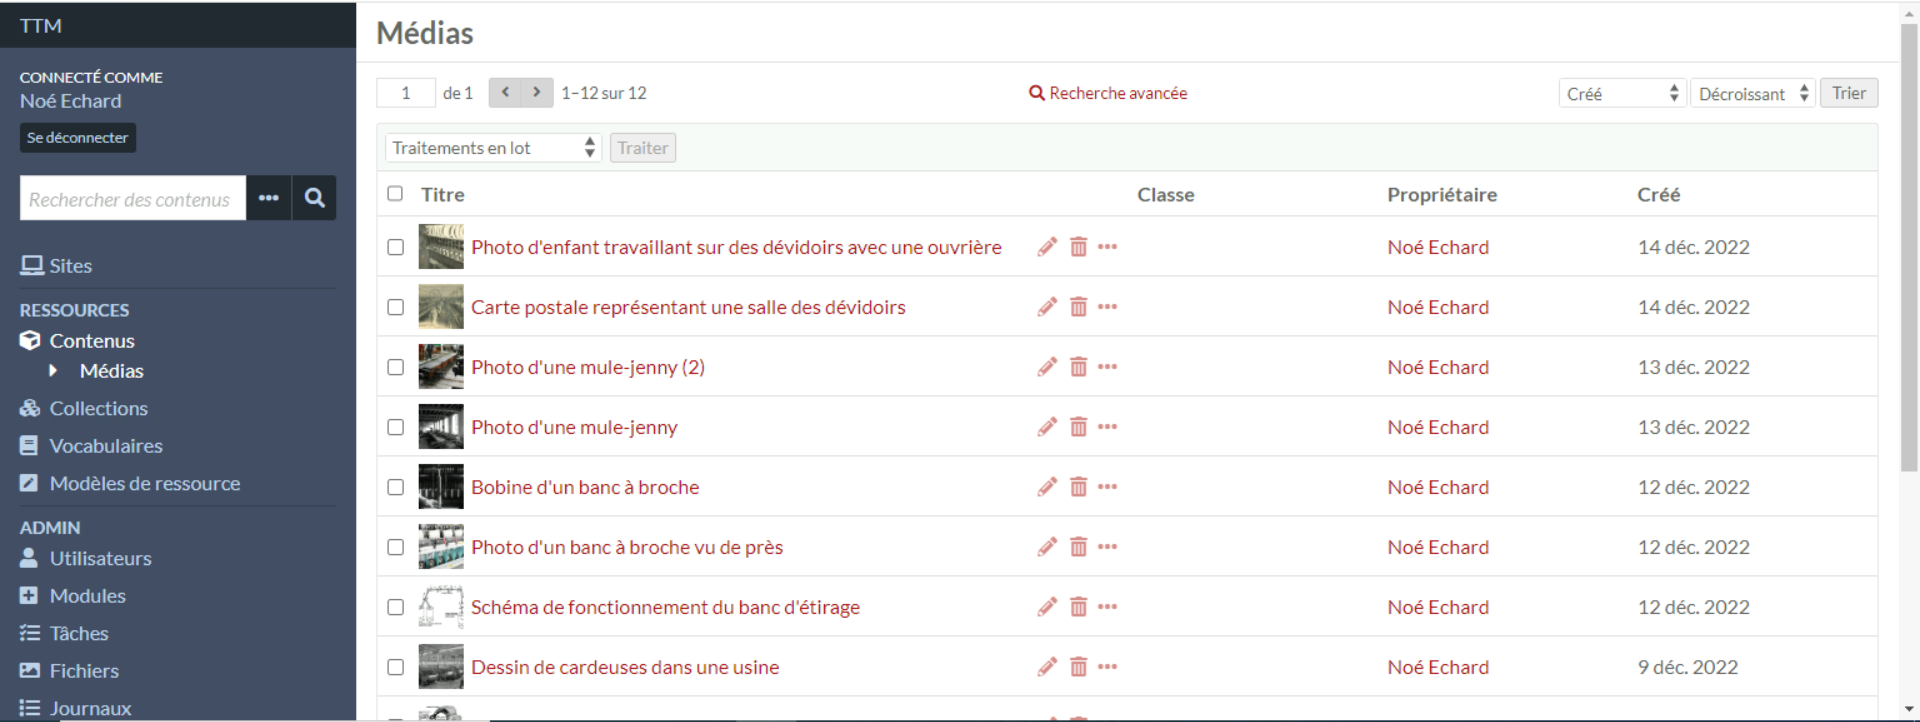
\includegraphics[width=1\textwidth]{assets/omeka/onglet_media_omeka.png}
    \caption{Capture d'écran de l'onglet medias de Omeka-S}
    \label{fig:pageMediasOmeka}
\end{figure}

\addcontentsline{toc}{section}{Omeka-S - Onglet "Modèles de ressources"}
\begin{figure} [H]
    \centering
    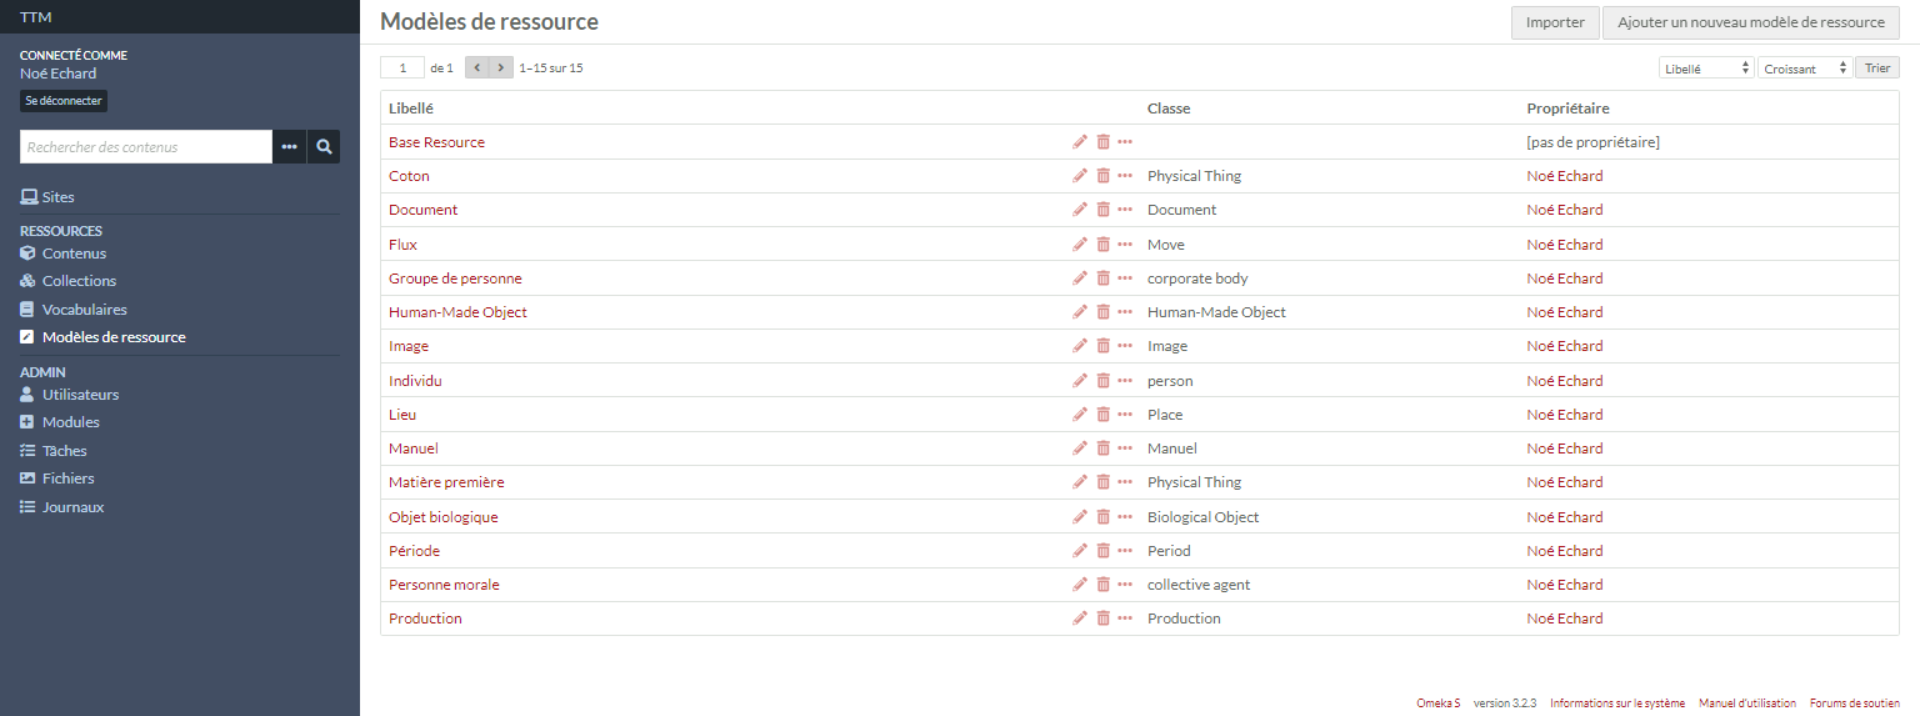
\includegraphics[width=1\textwidth]{assets/omeka/onglet_modele_ressource_omeka.png}
    \caption{Capture d'écran de l'onglet modèle de ressources de Omeka-S}
    \label{fig:pageModRessourceOmeka}
\end{figure}

\addcontentsline{toc}{section}{Omeka-S - Onglet "Users"}
\begin{figure} [H]
    \centering
    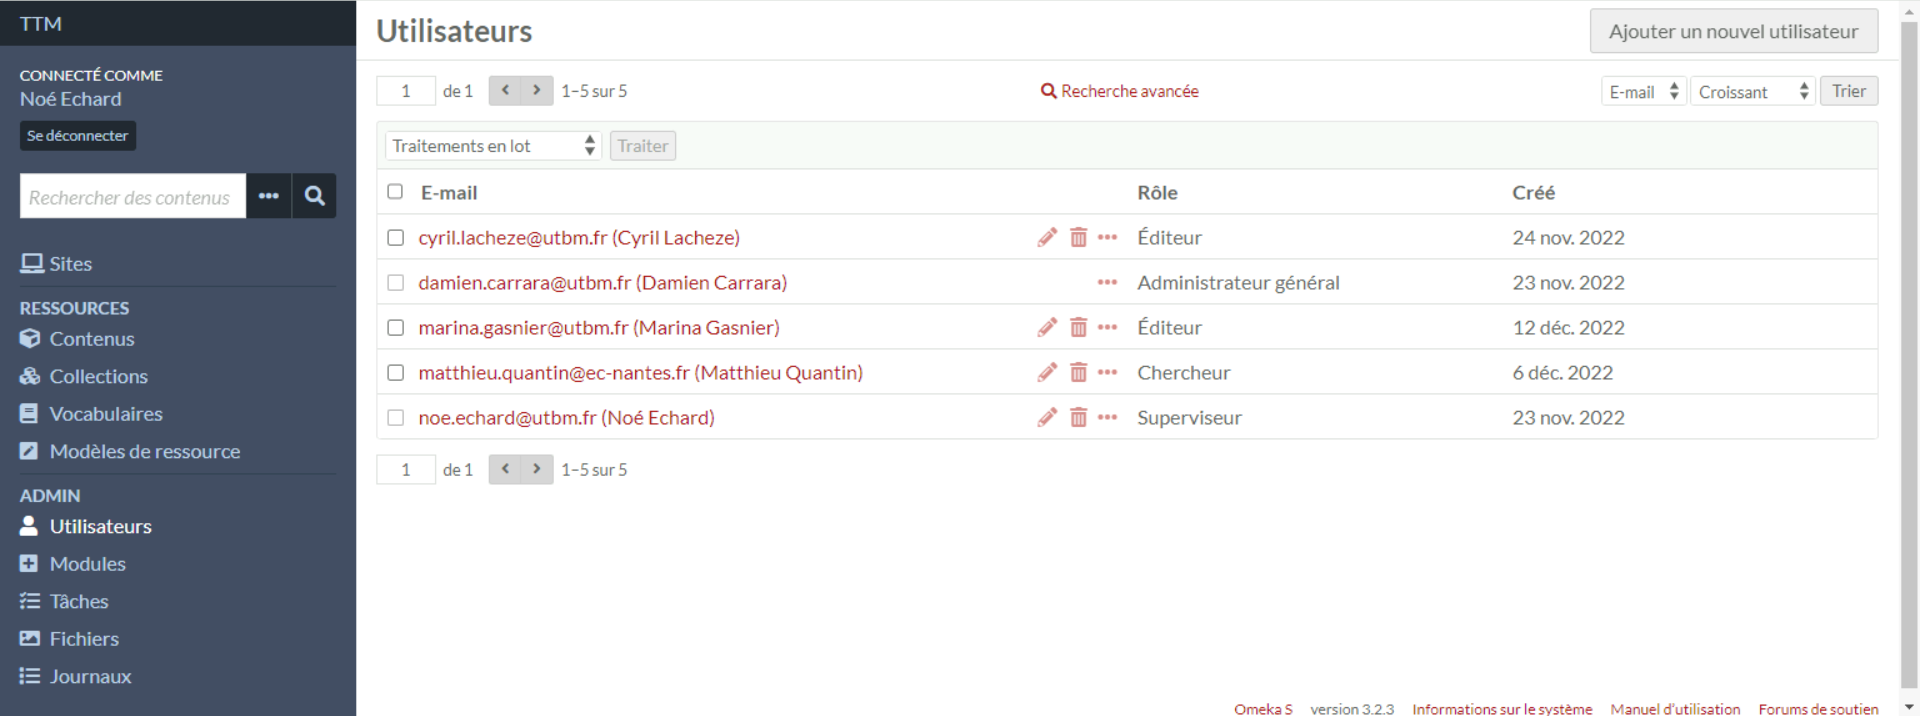
\includegraphics[width=1\textwidth]{assets/omeka/onglet_users_omeka.png}
    \caption{Capture d'écran de l'onglet users de Omeka-S}
    \label{fig:pageUsersOmeka}
\end{figure}

% AJOUTER DES SCREENS DU SITE WEB
% AJOUTER DES SCREENS DES FICHIERS DE L'ONTOLOGIE/SHACL
% AJOUTER DES SCREENS DU PROJET UNITY